\begin{frame}{Despliegue de los modelos en un entorno real}
El despliegue efectivo de estos modelos contribuye a mejorar la seguridad en redes mediante la automatización de la detección de conexiones malignas, permitiendo respuestas rápidas y reducidir el número de falsos positivos y negativos. La diferenciación entre múltiples tipos de conexiones malignas aporta un valor añadido para estrategias de mitigación específicas y optimización de recursos.

\begin{figure}[H]
    \centering
    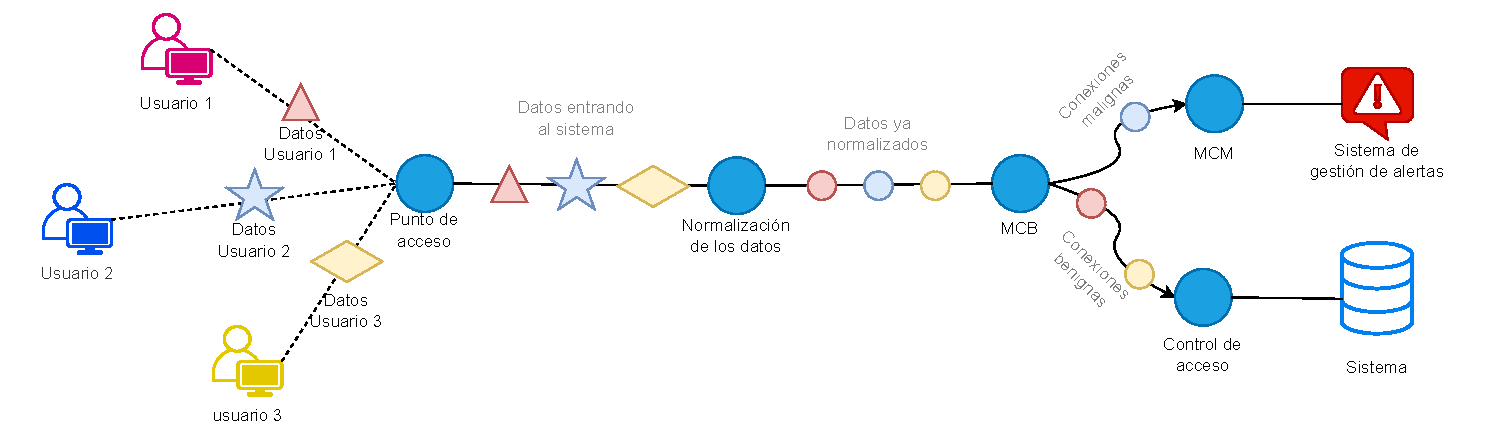
\includegraphics[width=1\textwidth]{../Memoria/img/despliegue/despliegue.pdf}
    \caption{Ejemplo de despliegue de los modelos en un sistema informático.}
    \label{fig:despliegue}
\end{figure}

\end{frame}